\documentclass[12pt]{article}
\usepackage[utf8]{inputenc}
\usepackage{array}
\usepackage{xcolor}
\usepackage{graphicx}
\usepackage{mathtools}
\usepackage{amsmath}
\usepackage{multicol}
\usepackage{eqnarray}
\usepackage{wrapfig}
\usepackage{siunitx}


\usepackage{natbib}
\usepackage{hyperref}
\hypersetup{
	colorlinks=true,
	linkcolor=black,
	filecolor=mangeta,      
	urlcolor=blue,
	pdftitle={Overleaf Example},
	pdfpagemode=FullScreen,
}

\usepackage[margin=0.6in]{geometry}

\title{52nd—24th INTERNATIONAL-RUDOLF ORTVAY \\ PROBLEM SOLVING CONTEST IN PHYSICS \\ Problem 15}
\author{Nguyen Thanh Long}
\date{\today}

	\newcommand{\para}{\setminus \setminus}

\begin{document}
	
\maketitle
	
\noindent We consider a thin pipe with a regular N-angle base with radius of the inscribed circle is $R$ and wall thickness is $\delta$ and Electrical resistivity $\gamma$. The mass of the magnet is $m$ and its magnetic dipole is $p$. For a long enough tube, the velocity of the magnet is $v$. We choose cylindrical coordinate system $(\rho,\theta,z)$ with the height $z=0$ is the coordinate of the magnet at $t=0$ (We only consider this proplem when the velocity of magnet is constant, so $t=0$ can be any time we want to choose). 
	
\noindent The magnetic vector potential at a position $(\rho,z)$ from the location of a point dipole is:
$$ \vec{A} = \frac{\mu_0}{4 \pi} \frac{ \vec{p} \times \vec{r} }{r^3} = \frac{\mu_0 m \rho}{4 \pi \left[ \rho^2 + \left(z+vt \right)^2 \right]^{\frac{3}{2}}} \hat{\theta}.$$ 

\noindent The electric field of that point will be:
$$ \vec{E} = - \frac{ d \vec{A} }{dt} = \frac{3 \mu_0 m v \rho \left( z + vt \right)}{4 \pi \left[ \rho^2 + \left(z+vt \right)^2 \right]^{\frac{5}{2}}} \hat{\theta} .$$

\noindent With the rectangle wall of pipe, we will divide into 2 components: parallel to the surface and perpendicular to the surface. With the paralled component, the current density is the same as cylindrical tubes, we have: $j_t = \frac{E_t}{\gamma}$. But with the perpendicular component, when the magnet is falling, the current density will create the surface charge density $\sigma$ at two surface of tube. This surface charge density at two surface will create the new electric field $\frac{\sigma}{\varepsilon_0}$, so the paralled component of current density is $j_n = \frac{1}{\gamma} \left( E_n - \frac{\sigma}{\varepsilon_0} \right)$.

\begin{figure}[!htb]
	\centering
	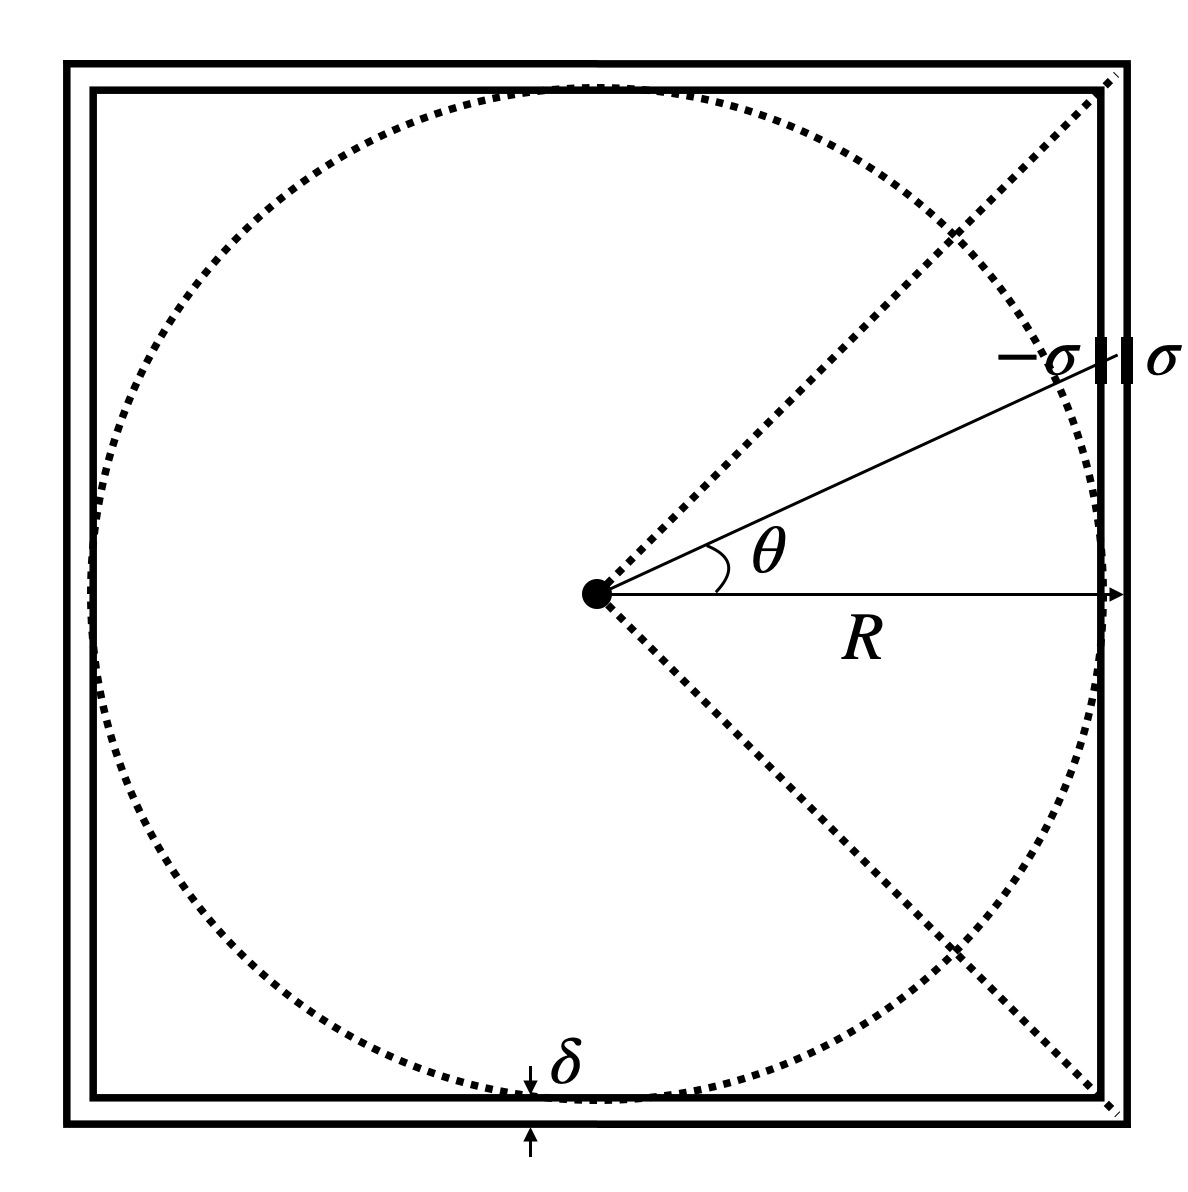
\includegraphics[width=0.3\textwidth]{Fig P15.png}
	\caption{ The pipe $N = 4$.}
	\label{fig1}
\end{figure}	

\noindent In the regular N-angle, we consider a edge from $\theta=-\frac{\pi}{N}$ to $\theta=\frac{\pi}{N}$. The radius of a point at $\theta$ is $\rho = \frac{R}{\cos \theta}$. Therefore, we have two equations of the current density at a point $(\theta, z)$:

\begin{align}
    j_t (\theta,z) & = \frac{E_t}{\gamma} = \frac{3 \mu_0 m v R \left( z + vt \right) }{4 \pi \gamma \left[ \left( \frac{R}{\cos \theta} \right)^2 + \left( z + vt \right)^2 \right]^{\frac{5}{2}} } . \label{eq1} \\
	j_n & = \frac{1}{\gamma} \left( E_n - \frac{\sigma}{\varepsilon_0} \right) . \label{eq2}
\end{align}	
	
\noindent Derivatives with respect to time with equation (\ref{eq2}), we have:
\begin{align*}
	\frac{ d j_n }{dt} & = \frac{1}{\gamma} \frac{d E_n}{dt} - \frac{1}{\gamma \varepsilon_0} j_n \\
	\Leftrightarrow \frac{d}{dt} \left( j_n e^{\frac{t}{\gamma \varepsilon_0}} - \frac{E_n}{\gamma} e^{\frac{t}{\gamma \varepsilon_0}} \right) & = - \frac{E_n}{\gamma^2 \varepsilon_0} e^{\frac{t}{\gamma \varepsilon_0}} \\
	\Rightarrow j_n & = \frac{E_n}{\gamma} - e^{-\frac{t}{\gamma \varepsilon_0}} \int \frac{E_n}{\gamma^2 \varepsilon_0} e^{\frac{t}{\gamma \varepsilon_0}} dt .
\end{align*}	

\noindent At $t = - \infty$, $j_n = 0$ and $E_n = 0$, so we will have: 
$$ j_n (\theta,z) = \frac{3 \mu_0 m v R \left( z + vt \right) \tan \theta }{4 \pi \gamma \left[ \left( \frac{R}{\cos \theta} \right)^2 + \left( z + vt \right)^2 \right]^{\frac{5}{2}} } - e^{-\frac{t}{\gamma \varepsilon_0}} \int_{-\infty}^t \frac{3 \mu_0 m v R \left( z + vt \right) \tan \theta }{4 \pi \gamma^2 \varepsilon_0 \left[ \left( \frac{R}{\cos \theta} \right)^2 + \left( z + vt \right)^2 \right]^{\frac{5}{2}} } e^{\frac{t}{\gamma \varepsilon_0}} dt .$$

\noindent Because when system reaches steady state we have $ \sigma(z,t) = \sigma (z + v \Delta t, t + \Delta t)$, then we can say that total energy of electric field is conservation. So all of work by gravity is used to heat dissipation on the resistor. Therefore, that power is:
\begin{align*}
	 P = mgv & = \int \gamma j^2 dV \\
	 & = \int_{-\infty}^{\infty} \left[ N \int_{-\frac{\pi}{N}}^{\frac{\pi}{N}} \gamma \left( j_t^2 + j_n^2 \right) \frac{R d \theta}{\cos^2 \theta} \delta \right] dz .
\end{align*} 

\noindent Remember that $P$ doesn't depend on $t$, so we choose $t=0$ to calculate the next part. Let $x = \frac{z}{R}$ We let the function $f(\theta,z)$ is:
$$f(\theta,x) = \int_{-\infty}^0 \frac{x + \frac{vt}{R}}{\gamma \varepsilon_0 \left[ \left( \frac{1}{\cos \theta} \right)^2 + \left(x + \frac{vt}{R} \right)^2 \right]^{\frac{5}{2}} } e^{\frac{t}{\gamma \varepsilon_0}} dt .$$

\noindent So we write the equation of power again:

\begin{align*}
	mg & = \frac{9 \mu_0^2 N p^2 v \delta}{16 \pi^2 \gamma R^4} \int_{-\infty}^{\infty} \int_{-\frac{\pi}{N}}^{\frac{\pi}{N}} \left[ \frac{x^2}{\left[ \left( \frac{1}{\cos \theta} \right)^2 + x^2 \right]^5} + \left( \frac{x \tan \theta}{\left[ \left( \frac{1}{\cos \theta} \right)^2 + x^2 \right]^{\frac{5}{2}}} - f(\theta, x) \right)^2 \right] \frac{d \theta}{\cos^2 \theta} dx . 
\end{align*}

\noindent Although we can't calculate this intergral by the hand, we can guess that it will be a function of $N$ and $\frac{v \gamma \varepsilon_0}{R}$. Set all the intergral is $F \left(N, \frac{v \gamma \varepsilon_0}{R} \right)$. We can see that our velocity of magnet is the solution of the equation:
$$ \frac{16 \pi^2 \gamma R^4 mg}{9 \mu_0^2 p^2 N \delta} = v F \left(N, \frac{v \gamma \varepsilon_0}{R} \right) .$$ 
	
\noindent In reality, the resistivity of a conductive material is $\gamma \sim 10^{-8} \si{\Omega \cdot m} $ and with proper time of this system is $\tau = \gamma \varepsilon_0 \sim 10^{-19} \si{s} $ (very small), so we also can assume that the perpendicular component of current density is very small and we can ignore it. In that case:
$$ F(N) = \int_{-\infty}^{\infty} \int_{-\frac{\pi}{N}}^{\frac{\pi}{N}} \frac{x^2}{\left[ \left( \frac{1}{\cos \theta} \right)^2 + x^2 \right]^5 } \frac{d \theta}{\cos^2 \theta} dx = \frac{5 \pi}{64} \left[ \sin \left( \frac{\pi}{N} \right) - \frac{2}{3} \sin^3 \left( \frac{\pi}{N} \right) + \frac{1}{5} \sin^5 \left( \frac{\pi}{N} \right) \right] .$$
	
\noindent Thus, the velocity of magnet is:
$$ v (N) = \frac{1024 mg \gamma R^4}{45 \mu_0^2 p^2 \delta }
\frac{ \frac{\pi}{N} }{ \sin \left( \frac{\pi}{N} \right) - \frac{2}{3} \sin^3 \left( \frac{\pi}{N} \right) + \frac{1}{5} \sin^5 \left( \frac{\pi}{N} \right) } .$$

\noindent Let's check this solution, with cylindrical tube, $N \Rightarrow \infty$, the velocity of magnet is: $ v (\infty) = \frac{1024 mg \gamma R^4}{45 \mu_0^2 p^2 \delta } $ (the same as a lot of previous calculations \cite{doi:10.1119/1.2203645} ). For the other values, we set a function $g(N)$ so that $v(N) = g(N) v(\infty)$ and we have this tabular:

\begin{center}
\begin{tabular}{| >{\centering\arraybackslash}m{1cm}| >{\centering\arraybackslash}m{1cm}| >{\centering\arraybackslash}m{1cm}| >{\centering\arraybackslash}m{1cm}| >{\centering\arraybackslash}m{1cm}| >{\centering\arraybackslash}m{1cm}| >{\centering\arraybackslash}m{1cm}| >{\centering\arraybackslash}m{1cm}|}
\hline 
$N$ & $\infty$  & $3$ & $4$ & $5$ & $6$ & $7$ & $8$ \\
\hline
$g(N)$ & $1$ & $1.974$ & $1.550$ & $1.347$ & $1.238$ & $1.173$ & $1.132$ \\
\hline
\end{tabular}
\end{center}

\bibliographystyle{plain}
\begin{thebibliography}{1}
	\bibitem{doi:10.1119/1.2203645} Yan Levin, Fernando L. da Silveira, and Felipe B. Rizzato. Electromagnetic braking: A simplequantitative model. \textit{American Journal of Physics}, 74(9):815–817, 2006.
\end{thebibliography}	








\end{document}